\documentclass[a4paper,11pt]{article}
\usepackage[a4paper, margin=8em]{geometry}

% usa i pacchetti per la scrittura in italiano
\usepackage[french,italian]{babel}
\usepackage[T1]{fontenc}
\usepackage[utf8]{inputenc}
\frenchspacing 

% usa i pacchetti per la formattazione matematica
\usepackage{amsmath, amssymb, amsthm, amsfonts}

% usa altri pacchetti
\usepackage{gensymb}
\usepackage{hyperref}
\usepackage{standalone}

\usepackage{colortbl}

\usepackage{xstring}
\usepackage{karnaugh-map}

% imposta il titolo
\title{Appunti Sistemi Operativi}
\author{Luca Seggiani}
\date{2025}

% imposta lo stile
% usa helvetica
\usepackage[scaled]{helvet}
% usa palatino
\usepackage{palatino}
% usa un font monospazio guardabile
\usepackage{lmodern}

\renewcommand{\rmdefault}{ppl}
\renewcommand{\sfdefault}{phv}
\renewcommand{\ttdefault}{lmtt}

% circuiti
\usepackage{circuitikz}
\usetikzlibrary{babel}

% testo cerchiato
\newcommand*\circled[1]{\tikz[baseline=(char.base)]{
            \node[shape=circle,draw,inner sep=2pt] (char) {#1};}}

% disponi il titolo
\makeatletter
\renewcommand{\maketitle} {
	\begin{center} 
		\begin{minipage}[t]{.8\textwidth}
			\textsf{\huge\bfseries \@title} 
		\end{minipage}%
		\begin{minipage}[t]{.2\textwidth}
			\raggedleft \vspace{-1.65em}
			\textsf{\small \@author} \vfill
			\textsf{\small \@date}
		\end{minipage}
		\par
	\end{center}

	\thispagestyle{empty}
	\pagestyle{fancy}
}
\makeatother

% disponi teoremi
\usepackage{tcolorbox}
\newtcolorbox[auto counter, number within=section]{theorem}[2][]{%
	colback=blue!10, 
	colframe=blue!40!black, 
	sharp corners=northwest,
	fonttitle=\sffamily\bfseries, 
	title=Teorema~\thetcbcounter: #2, 
	#1
}

% disponi definizioni
\newtcolorbox[auto counter, number within=section]{definition}[2][]{%
	colback=red!10,
	colframe=red!40!black,
	sharp corners=northwest,
	fonttitle=\sffamily\bfseries,
	title=Definizione~\thetcbcounter: #2,
	#1
}

% disponi codice
\usepackage{listings}
\usepackage[table]{xcolor}

\definecolor{codegreen}{rgb}{0,0.6,0}
\definecolor{codegray}{rgb}{0.5,0.5,0.5}
\definecolor{codepurple}{rgb}{0.58,0,0.82}
\definecolor{backcolour}{rgb}{0.95,0.95,0.92}

\lstdefinestyle{codestyle}{
		backgroundcolor=\color{black!5}, 
		commentstyle=\color{codegreen},
		keywordstyle=\bfseries\color{magenta},
		numberstyle=\sffamily\tiny\color{black!60},
		stringstyle=\color{green!50!black},
		basicstyle=\ttfamily\footnotesize,
		breakatwhitespace=false,         
		breaklines=true,                 
		captionpos=b,                    
		keepspaces=true,                 
		numbers=left,                    
		numbersep=5pt,                  
		showspaces=false,                
		showstringspaces=false,
		showtabs=false,                  
		tabsize=2
}

\lstdefinestyle{shellstyle}{
		backgroundcolor=\color{black!5}, 
		basicstyle=\ttfamily\footnotesize\color{black}, 
		commentstyle=\color{black}, 
		keywordstyle=\color{black},
		numberstyle=\color{black!5},
		stringstyle=\color{black}, 
		showspaces=false,
		showstringspaces=false, 
		showtabs=false, 
		tabsize=2, 
		numbers=none, 
		breaklines=true
}


\lstdefinelanguage{assembler}{ 
  keywords={AAA, AAD, AAM, AAS, ADC, ADCB, ADCW, ADCL, ADD, ADDB, ADDW, ADDL, AND, ANDB, ANDW, ANDL,
        ARPL, BOUND, BSF, BSFL, BSFW, BSR, BSRL, BSRW, BSWAP, BT, BTC, BTCB, BTCW, BTCL, BTR, 
        BTRB, BTRW, BTRL, BTS, BTSB, BTSW, BTSL, CALL, CBW, CDQ, CLC, CLD, CLI, CLTS, CMC, CMP,
        CMPB, CMPW, CMPL, CMPS, CMPSB, CMPSD, CMPSW, CMPXCHG, CMPXCHGB, CMPXCHGW, CMPXCHGL,
        CMPXCHG8B, CPUID, CWDE, DAA, DAS, DEC, DECB, DECW, DECL, DIV, DIVB, DIVW, DIVL, ENTER,
        HLT, IDIV, IDIVB, IDIVW, IDIVL, IMUL, IMULB, IMULW, IMULL, IN, INB, INW, INL, INC, INCB,
        INCW, INCL, INS, INSB, INSD, INSW, INT, INT3, INTO, INVD, INVLPG, IRET, IRETD, JA, JAE,
        JB, JBE, JC, JCXZ, JE, JECXZ, JG, JGE, JL, JLE, JMP, JNA, JNAE, JNB, JNBE, JNC, JNE, JNG,
        JNGE, JNL, JNLE, JNO, JNP, JNS, JNZ, JO, JP, JPE, JPO, JS, JZ, LAHF, LAR, LCALL, LDS,
        LEA, LEAVE, LES, LFS, LGDT, LGS, LIDT, LMSW, LOCK, LODSB, LODSD, LODSW, LOOP, LOOPE,
        LOOPNE, LSL, LSS, LTR, MOV, MOVB, MOVW, MOVL, MOVSB, MOVSD, MOVSW, MOVSX, MOVSXB,
        MOVSXW, MOVSXL, MOVZX, MOVZXB, MOVZXW, MOVZXL, MUL, MULB, MULW, MULL, NEG, NEGB, NEGW,
        NEGL, NOP, NOT, NOTB, NOTW, NOTL, OR, ORB, ORW, ORL, OUT, OUTB, OUTW, OUTL, OUTSB, OUTSD,
        OUTSW, POP, POPL, POPW, POPB, POPA, POPAD, POPF, POPFD, PUSH, PUSHL, PUSHW, PUSHB, PUSHA, 
				PUSHAD, PUSHF, PUSHFD, RCL, RCLB, RCLW, MOVSL, MOVSB, MOVSW, STOSL, STOSB, STOSW, LODSB, LODSW,
				LODSL, INSB, INSW, INSL, OUTSB, OUTSL, OUTSW
        RCLL, RCR, RCRB, RCRW, RCRL, RDMSR, RDPMC, RDTSC, REP, REPE, REPNE, RET, ROL, ROLB, ROLW,
        ROLL, ROR, RORB, RORW, RORL, SAHF, SAL, SALB, SALW, SALL, SAR, SARB, SARW, SARL, SBB,
        SBBB, SBBW, SBBL, SCASB, SCASD, SCASW, SETA, SETAE, SETB, SETBE, SETC, SETE, SETG, SETGE,
        SETL, SETLE, SETNA, SETNAE, SETNB, SETNBE, SETNC, SETNE, SETNG, SETNGE, SETNL, SETNLE,
        SETNO, SETNP, SETNS, SETNZ, SETO, SETP, SETPE, SETPO, SETS, SETZ, SGDT, SHL, SHLB, SHLW,
        SHLL, SHLD, SHR, SHRB, SHRW, SHRL, SHRD, SIDT, SLDT, SMSW, STC, STD, STI, STOSB, STOSD,
        STOSW, STR, SUB, SUBB, SUBW, SUBL, TEST, TESTB, TESTW, TESTL, VERR, VERW, WAIT, WBINVD,
        XADD, XADDB, XADDW, XADDL, XCHG, XCHGB, XCHGW, XCHGL, XLAT, XLATB, XOR, XORB, XORW, XORL},
  keywordstyle=\color{blue}\bfseries,
  ndkeywordstyle=\color{darkgray}\bfseries,
  identifierstyle=\color{black},
  sensitive=false,
  comment=[l]{\#},
  morecomment=[s]{/*}{*/},
  commentstyle=\color{purple}\ttfamily,
  stringstyle=\color{red}\ttfamily,
  morestring=[b]',
  morestring=[b]"
}

\lstset{language=assembler, style=codestyle}

% disponi sezioni
\usepackage{titlesec}

\titleformat{\section}
	{\sffamily\Large\bfseries} 
	{\thesection}{1em}{} 
\titleformat{\subsection}
	{\sffamily\large\bfseries}   
	{\thesubsection}{1em}{} 
\titleformat{\subsubsection}
	{\sffamily\normalsize\bfseries} 
	{\thesubsubsection}{1em}{}

% tikz
\usepackage{tikz}

% float
\usepackage{float}

% grafici
\usepackage{pgfplots}
\pgfplotsset{width=10cm,compat=1.9}

% disponi alberi
\usepackage{forest}

\forestset{
	rectstyle/.style={
		for tree={rectangle,draw,font=\large\sffamily}
	},
	roundstyle/.style={
		for tree={circle,draw,font=\large}
	}
}

% disponi algoritmi
\usepackage{algorithm}
\usepackage{algorithmic}
\makeatletter
\renewcommand{\ALG@name}{Algoritmo}
\makeatother

% disponi numeri di pagina
\usepackage{fancyhdr}
\fancyhf{} 
\fancyfoot[L]{\sffamily{\thepage}}

\makeatletter
\fancyhead[L]{\raisebox{1ex}[0pt][0pt]{\sffamily{\@title \ \@date}}} 
\fancyhead[R]{\raisebox{1ex}[0pt][0pt]{\sffamily{\@author}}}
\makeatother

\begin{document}
% sezione (data)
\section{Lezione del 02-10-25}

% stili pagina
\thispagestyle{empty}
\pagestyle{fancy}

% testo
Continuiamo la discussione dei processi:

\subsubsection{Stato dei processi}
In un \textbf{S/O monoprogrammato} il processo può trovarsi in uno di due stati:

\begin{center}
	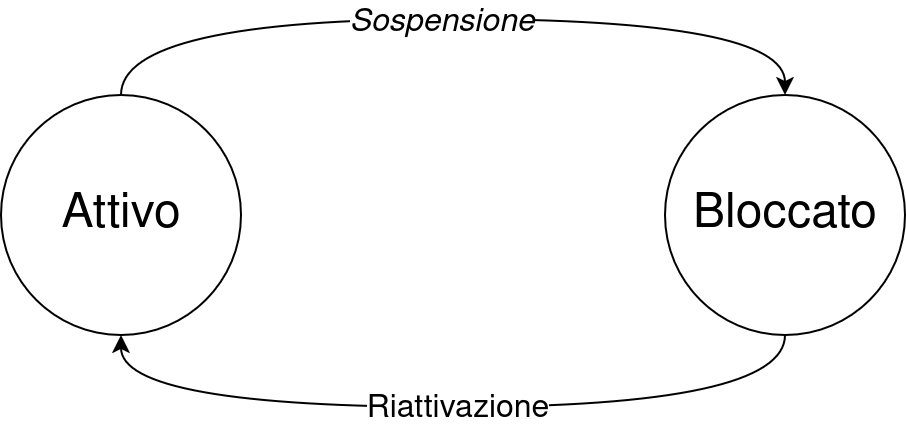
\includegraphics[scale=0.25]{../figures/proc_attivo_bloccato.png}
\end{center}

\begin{itemize}
	\item \textbf{Attivo}: il processo stato creato, è in esecuzione ed ha ancora istruzioni da eseguire. 

		\textit{Creare} un processo significa in primo luogo allocare le strutture dati che lo descrivono. In seguito, si deve allocare un po' di memoria al processo stesso per contenere i suoi dati (istruzioni, pila, ecc...) come visto in 4.6.
	Abbiamo però che allocare particolari descrittori al processo quando questo è l'unico in esecuzione sarebbe inutile: effettivamente un sistema monoprogrammato può essere tale solo se il processo in esecuzione è in qualche modo il S/O.

		A questo punto il processo è l'unico in esecuzione sulla CPU, e resterà tale fino alla fine del suo \textit{lifetime}.
		Dovrà però \textit{bloccarsi} se vuole accedere a risorse sistema: fara ciò usando una \textit{chiamata a sistema};

	\item \textbf{Bloccato}: il processo o qualche altro attore ha causato un qualche evento che ha determinato il passaggio di controllo al S/O (richiesta risorse di I/O, di risorse logiche, interruzioni esterne, ecc...).

		A questo punto sarà nuovamente un evento esterno (interruzione esterna, azione dell'utente) a riportare in esecuzione un processo, creandone uno nuovo se lo scorso aveva terminato, o rimettendo il corrente in esecuzione se si era bloccao su una operazione di I/O o simile.

		Notiamo che la memoria del processo potrebbe cambiare anche questo è bloccato: ad esempio se si hanno dispositivi che operano in DMA. 
\end{itemize}

La transizione fra attivo e bloccato è detta \textit{sospensione}, mentre fra bloccato e attivo è è detta \textit{riattivazione}.

Possiamo dire che gli stati \textit{attivo} e \textit{bloccato} sono in qualche modo in corrispondenza con le fasi descritte in 2.1.4 di \textbf{CPU-Burst} e \textbf{I/O-Burst}.

\par\bigskip

Se il numero di CPU è minore del numero dei processi, cioè in un sistema \textbf{monoprocessore}, ci dotiamo di più stati:

\begin{center}
	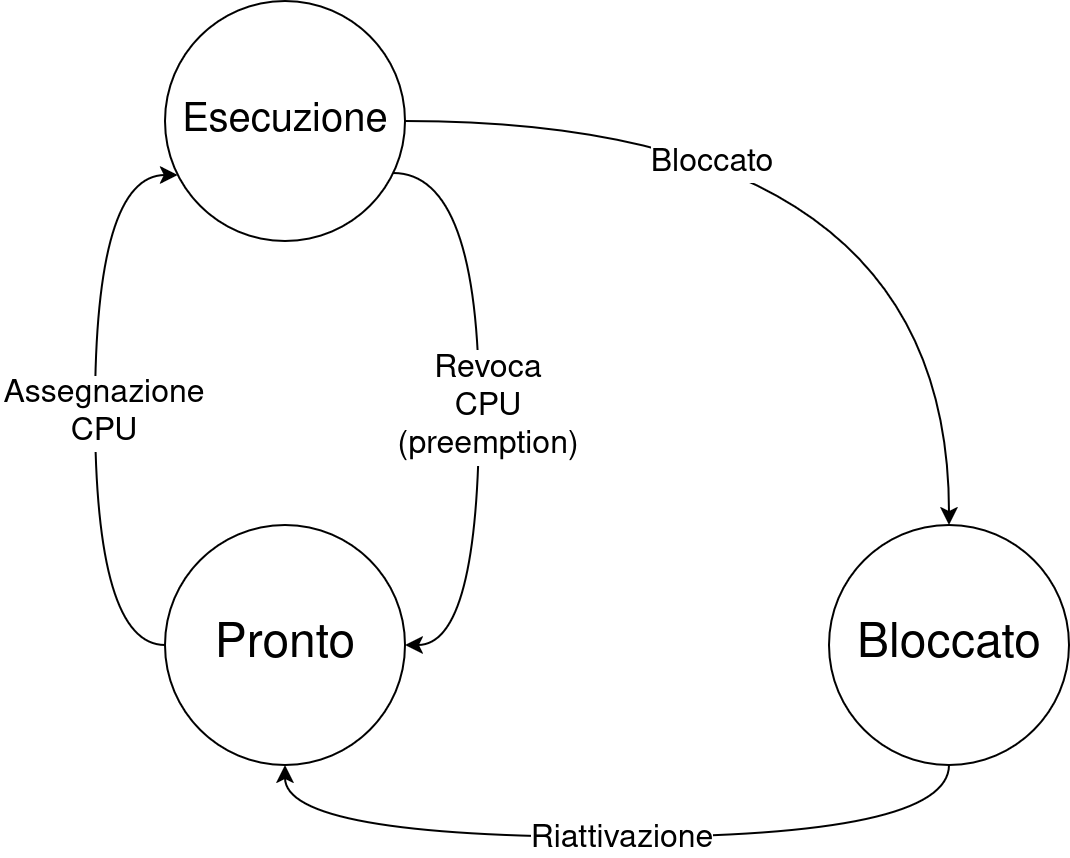
\includegraphics[scale=0.25]{../figures/proc_esecuzione_pronto_bloccato.png}
\end{center}

\begin{itemize}
	\item \textbf{Pronto}: in questo caso il processo è in attesa del tempo del processore. Abbiamo che nella maggior parte delle implementazioni questo stato è rappresentato da una \textit{coda} di descrittori di processo, la cosiddetta \textbf{coda pronti} (utile per implementare politiche prioritarie $\leftrightarrow$ code prioritarie);
	\item \textbf{Esecuzione}: il processo è in esecuzione sulla CPU;
	\item \textbf{Bloccato}: il processo è in attesa, come nell'esempio precedente. 

		In questo caso, come nel precedente, la memoria processo potrebbe essere modificata da dispositivi in DMA.
	Potrebbero poi essere modificati, in particolari situazioni, i descrittori di processo: magari a causa di operazioni di altri processi col S/O (pipe fra processi, ecc...).	
\end{itemize}

La transizione da pronto e esecuzione è detta \textit{assegnazione CPU}, mentre la contraria è detta \textit{revoca CPU}, o in inglese \textbf{preemption}.
Notiamo che quest'ultima transizione non è prevista da tutti i sistemi.

L'operazione di assegnazione CPU è eseguita da un componente del S/O detto \textbf{scheduler}. Lo scheduler viene eseguito quando il processo in esecuzione cambia stato, quindi in caso di \textit{revoca CPU} o \textit{sospensione}: sostanzialmente ogni volta che si richiede un nuovo processo da mettere in esecuzione.
Questo comprende anche la situazione in cui il processo corrente \textit{termina}.

Abbiamo poi che la transizioni allo stato bloccato sono le stesse dell'esempio precedente, con l'unica differenza che la \textit{riattivazione} del processo non lo mette in esecuzione ma nello stato \textit{pronto}.

C'è inoltre un'altro stato, oltre a quello di \textit{terminazione} prima accennato, di cui dobbiamo tener conto: quello in cui il processo viene \textit{creato}, cioè la transizione di un nuovo processo allo stato di \textit{pronto} (detta \textit{attivazione}):

\begin{center}
	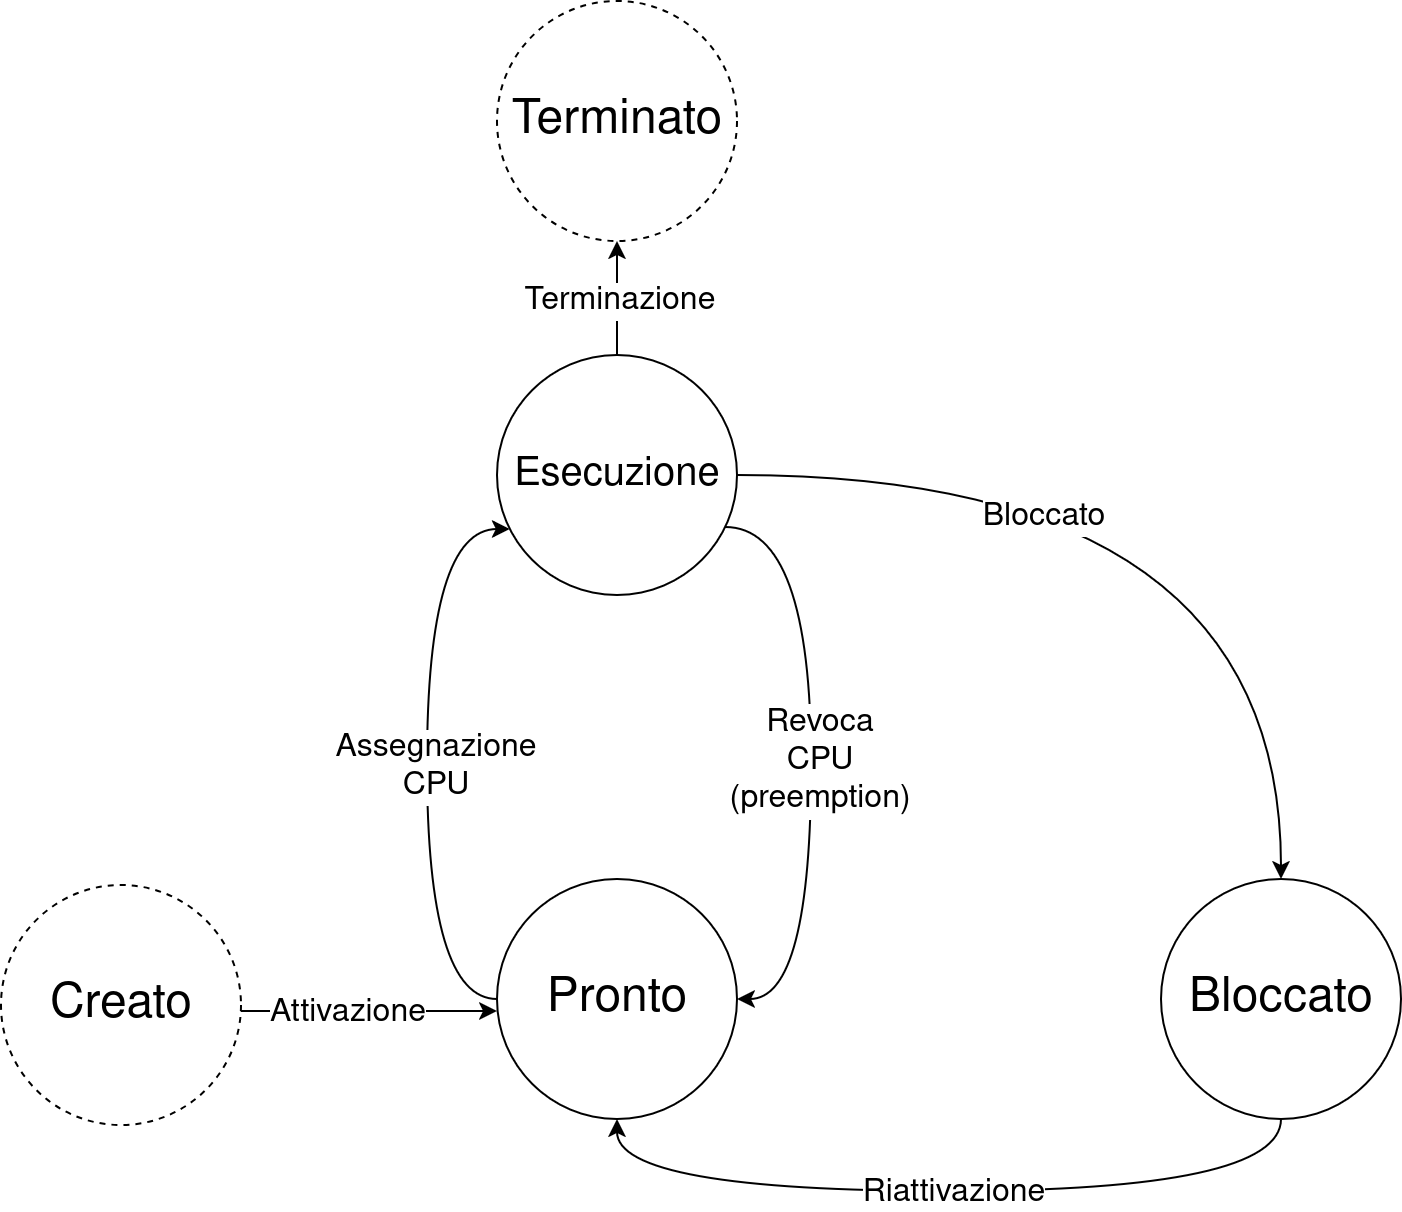
\includegraphics[scale=0.25]{../figures/proc_creato_esecuzione_pronto_bloccato_terminato.png}
\end{center}

In questo caso possiamo anticipare che in S/O che adottano politiche \textit{prioritarie} allo scheduling potrebbe essere necessario eseguire lo scheduler (per mettere in esecuzione un nuovo processo di priorità più alta).

\subsubsection{Descrittori di processo}
Abbiamo introdotto come la gestione dei processi bisogna di apposite strutture dati dette \textit{descrittori} di processo (in inglese \textbf{PCB}, \textit{Process Control Block}).

Questa dovrà associare ad ogni processo:
\begin{itemize}
	\item Nome del processo: questo è il solito \textbf{PID} (\textit{Process IDentifier}), ed identifica univocamente ogni processo. Richiedere che i PID siano univici è una \textit{politica} che li trasforma in una \textit{risorsa}: l'S/O dovrà impegnarsi a gestire i PID in modo che non avvengano collisioni;
	\item Stato del processo: codifica uno degli stati definiti prima;
	\item Modalità di servizio: questo riguarda la priorità (se implementata) o il tipo di scheduling che si usa per gestire il processo;
	\item Informazioni sulla gestione della memoria: conterrà puntatori alla memoria dedicata al processo;
	\item Contesto del processo: l'immagine dei registri all'ultima sospensione del processo;
	\item Utilizzo delle risorse: conterrà puntatori alle risorse logiche e fisiche a cui ha accesso il processo;
	\item Idefntificazione del processo successivo: questo serve semplicemente ad implementare, come abbiamo accennato, le code prioritarie di processi (come ad esempio la \textit{coda pronti}).
\end{itemize}

Una volta definito il descrittore di processo, potremo volerci fornire di:
\begin{itemize}
	\item La coda dei processi pronti;
	\item Una o più code per i processi bloccati (solitamente una coda è associata a una risorsa su cui i processi si bloccano);
	\item Un registro di qualche tipo che contiene il processo attualmente in esecuzione. 
\end{itemize}

\subsubsection{Cambio di contesto}
Il \textbf{cambio di contesto} è l'operazione attraverso cui l'uso del processore viene commutato da un processo all'altro.
Questo consiste in:
\begin{enumerate}
	\item Salvataggio del contesto del processo in esecuzione nel suo descrittore (cioè salvataggio di \textit{stato});
	\item Inserimento del descrittore di processo corrente in coda \textit{bloccati} o \textit{pronti}.
	\item Selezione di un nuovo processo da mettere in esecuzione e caricamento nel registro del descrittore del processo corrente (\textit{short term schedulilng});
	\item Caricamento del contesto del nuovo processo e cessione a questi del controllo. 
\end{enumerate}

Notiamo che per realizzare il cambio di contesto al S/O (che si occupa poi di portare avanti queste operazioni) abbiamo bisogno di funzionalità implementate in hardware: il "processo" S/O è semplicemente il processo in esecuzione al tempo del cambio, che è forzato a passare al contesto sistema nell'istante in cui si mette ad eseguire codice sistema.
Questo si riassume nella lista di operazioni ai passi (1) e (4).

Questo significa che per realizzare un S/O si necessita di un processore che implementi il cambio di contesto (x86 dal 286, ecc...). 

\par\smallskip

Possiamo iniziare ad approfondire il modo in cui indicizziamo il processo. Dal punto di vista concettuale, vorremo usare una tripla:
$$
S = < \text{PID}, \text{UID}, \text{GID} >
$$
composta da \textbf{PID} (\textit{Process IDentifier}, già visto), e \textbf{UID} e \textbf{GID} (\textit{User IDentifier} e \textit{Group IDentifier}), che rappresentano il proprietario del processo.

In caso di cambi di contesto al contesto sistema, quello che faremo è semplicemente cambiare UID e GID in modo da eseguire lo stesso processo, ma con privilegi diversi.

\subsubsection{Creazione e terminazione di processi}
Vediamo le operazioni che si possono svolgere sui processi.

Avremo che vorremo supportare \textit{gerarchie} di procssi, dove un processo (padre) può richiedere la creazione di un nuovo processo (figlio).
Questo significherà che ogni processo sarà figlio di un altro processa, e potra a sua volta essere padre di altri processi.
Chiaramente, le informazioni relative alle relazioni parentali saranno mantenute da S/O nei descrittori di processi.

Se un processo termina, di base:
\begin{itemize}
	\item Il padre può rilevare il suo stato di terminazione;
	\item Tutti i suoi figli terminano.
\end{itemize}

\subsubsection{Processi concorrenti}
Specifichiamo come più processi vengono eseguiti su una stessa macchina.
Abbiamo che questi possono alternarsi (\textit{interleaving}), tipico delle macchine a singolo processore, o eseguire effettivamente l'uno contemporaneamente all'altro. Questo è tipico delle macchine a più processori.

Nel caso di più processi in esecuzione contemporaneamente (diciamo processi \textit{concorrenti}) vengono a verificarsi alcune problematiche:
\begin{itemize}
	\item Processi \textbf{indipendenti}: se due processi $P1$ e $P2$ sono indipendenti, cioè non influenzano l'uno l'esecuzione dell'altra, dobbiamo assicurarci che questo resti vero, cioè dobbiamo risolvere il \textit{problema della riproducibilità}. Visto che le risorse sistema sono condivise, dobbiamo infatti assicurarci che non ci siano effetti collaterali sensibili da un processo o dall'altro.
	\item Processi \textbf{interagenti}: se due processi $P1$ e $P2$ devono interagire fra di loro, possono farlo in maniera \textit{esplicita} (per \textbf{cooperazione}), scambiandosi messaggi, o \textit{implicita} (per \textbf{competizione}), magari competendo per la stessa risorsa in mutua esclusione.
\end{itemize}


\end{document}
